%\documentclass[landscape]{article}
\documentclass[portrait]{article}
\usepackage[usenames]{color}

\usepackage{pgf}
\usepackage{tikz}

\usepackage{graphicx}

%\usepackage[brazil]{babel}
\usepackage[latin1]{inputenc}
\usepackage[T1]{fontenc}
\usepackage[all]{xy}

\usepackage {vmargin}           % para setar formato da página + facilmente

% Dimensões a ocupar na página (package Vmargin)
\setpapersize [portrait]{A4}
\setmarginsrb {25mm} % margem esquerda
              {25mm} % margem topo
              {20mm} % margem direita
              {20mm} % margem pé
              {2ex}  % altura do espaço para cabeçalho
              {2ex}  % espaço entre fim do cabeçalho e início do texto
              {2ex}  % altura do espaço para rodapé
              {2ex}  % espaço entre fim do texto e fim do rodapé

\usetikzlibrary{arrows,automata}
%\usetikzlibrary{positioning}
%\usetikzlibrary{arrows,decorations.pathmorphing,backgrounds,positioning,fit}
\usetikzlibrary{positioning,shapes,shadows,arrows}

%\definecolor{Peach}{rgb}{0,0.08,0.45}
\definecolor{Peach}{cmyk}{0,0.50,0.70,0}

\tikzset{
    state/.style={
           rectangle,
           fill = Peach!10,
           rounded corners,
%           draw = blue!50!black,
           very thick,
           minimum height = 2em,
           inner sep = 2pt,
           text centered,
           drop shadow,
           },
}
\tikzstyle{myarrow}=[->, >=open triangle 90, thick]

\begin{document}

\input ReachableDefinitions.tex
\clearpage

\input LiveVariable.tex
\clearpage

\input AvailableExpressions.tex
\clearpage

\input AnticipableExpressions.tex
\clearpage

\input PartiallyAvailableExpressions.tex
\clearpage

\input DeadVariable.tex
\clearpage

\input DefinitionsForCopyPropagation.tex
\clearpage

\input PartialRedundancy1.tex
\clearpage

\input ConstantPropagation.tex
\clearpage

\input Exemplos.tex

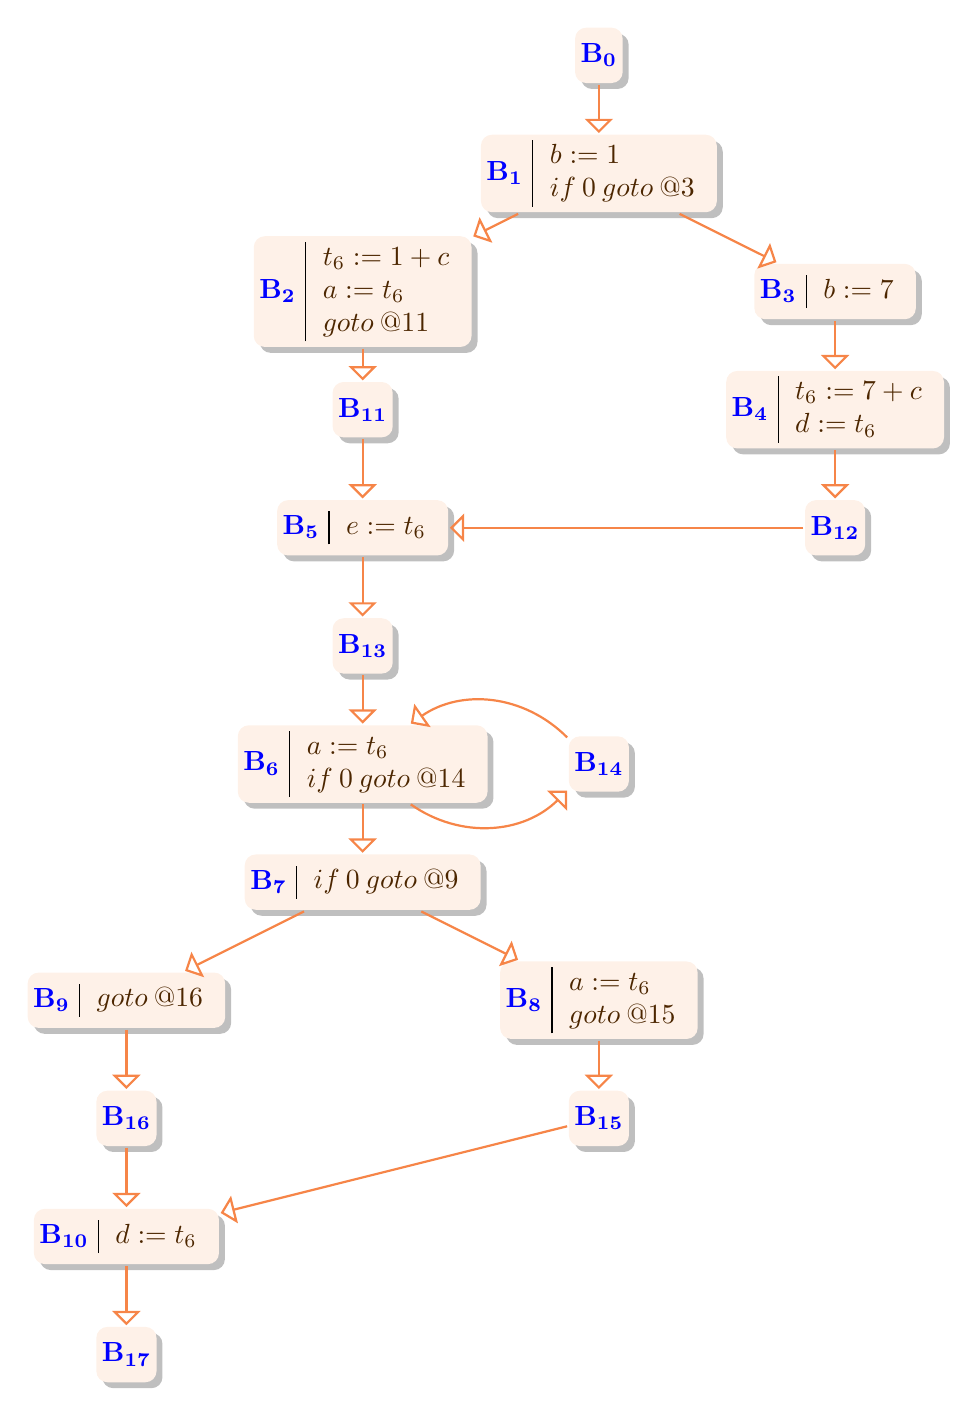
\begin{tikzpicture}[->,>=stealth']

 \node[state] (B0)
 {%
 \textcolor{blue}{\txt{$\mathbf{B_{0}}$}}
 };

\node[state,
  below of=B0,
  node distance=1.5cm,
  anchor=center] (B1)
 {%
 \textcolor{blue}{$\mathbf{B_{1}}$}
 \begin{tabular}{|l}
 {\color{orange!30!black}$b:=1$}\\
 {\color{orange!30!black}$if\:0\:goto\:@3$}
 \end{tabular}
 };

\node[
  right of=B1,
  node distance=3cm,
  anchor=center] (B1R)
 {};%
\node[
  left of=B1,
  node distance=3cm,
  anchor=center] (B1L)
 {};%

\node[state,
  below of=B1R,
  node distance=1.5cm,
  anchor=center] (B3)
 {%
 \textcolor{blue}{$\mathbf{B_{3}}$}
 \begin{tabular}{|l}
 {\color{orange!30!black}$b:=7$}
 \end{tabular}
 };

\node[state,
  below of=B3,
  node distance=1.5cm,
  anchor=center] (B4)
 {%
 \textcolor{blue}{$\mathbf{B_{4}}$}
 \begin{tabular}{|l}
 {\color{orange!30!black}$t_{6}:=7+c$}\\
 {\color{orange!30!black}$d:=t_{6}$}
 \end{tabular}
 };

\node[state,
  below of=B4,
  node distance=1.5cm,
  anchor=center] (B12)
 {%
 \textcolor{blue}{$\mathbf{B_{12}}$}
 };

\node[state,
  below of=B1L,
  node distance=1.5cm,
  anchor=center] (B2)
 {%
 \textcolor{blue}{$\mathbf{B_{2}}$}
 \begin{tabular}{|l}
 {\color{orange!30!black}$t_{6}:=1+c$}\\
 {\color{orange!30!black}$a:=t_{6}$}\\
 {\color{orange!30!black}$goto\:@11$}
 \end{tabular}
 };

\node[state,
  below of=B2,
  node distance=1.5cm,
  anchor=center] (B11)
 {%
 \textcolor{blue}{$\mathbf{B_{11}}$}
};

\node[state,
  below of=B11,
  node distance=1.5cm,
  anchor=center] (B5)
 {%
 \textcolor{blue}{$\mathbf{B_{5}}$}
 \begin{tabular}{|l}
 {\color{orange!30!black}$e:=t_{6}$}
 \end{tabular}
 };

\node[state,
  below of=B5,
  node distance=1.5cm,
  anchor=center] (B13)
 {%
 \textcolor{blue}{$\mathbf{B_{13}}$}
 };

\node[state,
  below of=B13,
  node distance=1.5cm,
  anchor=center] (B6)
 {%
 \textcolor{blue}{$\mathbf{B_{6}}$}
 \begin{tabular}{|l}
 {\color{orange!30!black}$a:=t_{6}$}\\
 {\color{orange!30!black}$if\:0\:goto\:@14$}
 \end{tabular}
 };

\node[state,
  right of=B6,
  node distance=3cm,
  anchor=center] (B14)
 {%
 \textcolor{blue}{$\mathbf{B_{14}}$}
 };

\node[state,
  below of=B6,
  node distance=1.5cm,
  anchor=center] (B7)
 {%
 \textcolor{blue}{$\mathbf{B_{7}}$}
 \begin{tabular}{|l}
 {\color{orange!30!black}$if\:0\:goto\:@9$}
 \end{tabular}
 };

\node[
  right of=B7,
  node distance=3cm,
  anchor=center] (B7R)
 {};%
\node[
  left of=B7,
  node distance=3cm,
  anchor=center] (B7L)
 {};%

\node[state,
  below of=B7L,
  node distance=1.5cm,
  anchor=center] (B9)
 {%
 \textcolor{blue}{$\mathbf{B_{9}}$}
 \begin{tabular}{|l}
 {\color{orange!30!black}$goto\:@16$}
 \end{tabular}
 };

\node[state,
  below of=B7R,
  node distance=1.5cm,
  anchor=center] (B8)
 {%
 \textcolor{blue}{$\mathbf{B_{8}}$}
 \begin{tabular}{|l}
 {\color{orange!30!black}$a:=t_{6}$}\\
 {\color{orange!30!black}$goto\:@15$}
 \end{tabular}
 };

\node[state,
  below of=B8,
  node distance=1.5cm,
  anchor=center] (B15)
 {%
 \textcolor{blue}{$\mathbf{B_{15}}$}
 };

\node[state,
  below of=B9,
  node distance=1.5cm,
  anchor=center] (B16)
 {%
 \textcolor{blue}{$\mathbf{B_{16}}$}
 };

\node[state,
  below of=B16,
  node distance=1.5cm,
  anchor=center] (B10)
 {%
 \textcolor{blue}{$\mathbf{B_{10}}$}
 \begin{tabular}{|l}
 {\color{orange!30!black}$d:=t_{6}$}
 \end{tabular}
 };

\node[state,
  below of=B10,
  node distance=1.5cm,
  anchor=center] (B17)
 {%
 \textcolor{blue}{$\mathbf{B_{17}}$}
 };

 \path (B0)     edge[color = Peach, myarrow] (B1)
 (B1)           edge[color = Peach, myarrow] (B2)
                edge[color = Peach, myarrow] (B3)
 (B2)           edge[color = Peach, myarrow] (B11)
 (B3)           edge[color = Peach, myarrow] (B4)
 (B4)           edge[color = Peach, myarrow] (B12)
 (B12)          edge[color = Peach, myarrow] (B5)
 (B11)          edge[color = Peach, myarrow] (B5)
 (B5)           edge[color = Peach, myarrow] (B13)
 (B13)          edge[color = Peach, myarrow] (B6)
 (B6)           edge[color = Peach, myarrow] (B7)
                edge[color = Peach, myarrow, bend right=40] (B14)
 (B14)          edge[color = Peach, myarrow, bend right=40] (B6)
 (B7)           edge[color = Peach, myarrow] (B8)
                edge[color = Peach, myarrow] (B9)
 (B8)           edge[color = Peach, myarrow] (B15)
 (B9)           edge[color = Peach, myarrow] (B16)
 (B15)          edge[color = Peach, myarrow] (B10)
 (B16)          edge[color = Peach, myarrow] (B10)
 (B10)          edge[color = Peach, myarrow] (B17)
;
\end{tikzpicture}


\begin{scriptsize}
\xy(0, 0)
	*++{\txt{$\mathbf{B_{0}}$\\}}*\frm{-,}="B0";
(0, -15)
	*++{\txt{$\mathbf{B_{1}}$\\$b:=1$\\$if\:0\:goto\:@3$\\}}*\frm{-,}="B1";
(-25, -30)
	*++{\txt{$\mathbf{B_{2}}$\\$t_{6}:=1+c$\\$a:=t_{6}$\\$goto\:@11$\\}}*\frm{-,}="B2";
(25, -30)
	*++{\txt{$\mathbf{B_{3}}$\\$b:=7$\\}}*\frm{-,}="B3";
(25, -45)
	*++{\txt{$\mathbf{B_{4}}$\\$t_{6}:=7+c$\\$d:=t_{6}$\\}}*\frm{-,}="B4";
(-25, -60)
	*++{\txt{$\mathbf{B_{5}}$\\$e:=t_{6}$\\}}*\frm{-,}="B5";
(-25, -90)
	*++{\txt{$\mathbf{B_{6}}$\\$a:=t_{6}$\\$if\:0\:goto\:@14$\\}}*\frm{-,}="B6";
(-50, -105)
	*++{\txt{$\mathbf{B_{7}}$\\$if\:0\:goto\:@9$\\}}*\frm{-,}="B7";
(-25, -120)
	*++{\txt{$\mathbf{B_{8}}$\\$a:=t_{6}$\\$goto\:@15$\\}}*\frm{-,}="B8";
(-75, -120)
	*++{\txt{$\mathbf{B_{9}}$\\$goto\:@16$\\}}*\frm{-,}="B9";
(-75, -150)
	*++{\txt{$\mathbf{B_{10}}$\\$d:=t_{6}$\\}}*\frm{-,}="B10";
(-25, -45)
	*++{\txt{$\mathbf{B_{11}}$\\}}*\frm{-,}="B11";
(25, -60)
	*++{\txt{$\mathbf{B_{12}}$\\}}*\frm{-,}="B12";
(-25, -75)
	*++{\txt{$\mathbf{B_{13}}$\\}}*\frm{-,}="B13";
(0, -105)
	*++{\txt{$\mathbf{B_{14}}$\\}}*\frm{-,}="B14";
(-25, -135)
	*++{\txt{$\mathbf{B_{15}}$\\}}*\frm{-,}="B15";
(-75, -135)
	*++{\txt{$\mathbf{B_{16}}$\\}}*\frm{-,}="B16";
(-75, -165)
	*++{\txt{$\mathbf{B_{17}}$\\}}*\frm{-,}="B17";
"B0";"B1" **@{.} ?> *{\dir{>}};
"B1";"B2" **@{.} ?> *{\dir{>}};
"B1";"B3" **@{.} ?> *{\dir{>}};
"B2";"B11" **@{.} ?> *{\dir{>}};
"B3";"B4" **@{.} ?> *{\dir{>}};
"B4";"B12" **@{.} ?> *{\dir{>}};
"B5";"B13" **@{.} ?> *{\dir{>}};
"B6";"B7" **@{.} ?> *{\dir{>}};
"B6";"B14" **@{.} ?> *{\dir{>}};
"B7";"B9" **@{.} ?> *{\dir{>}};
"B7";"B8" **@{.} ?> *{\dir{>}};
"B8";"B15" **@{.} ?> *{\dir{>}};
"B9";"B16" **@{.} ?> *{\dir{>}};
"B10";"B17" **@{.} ?> *{\dir{>}};
"B11";"B5" **@{.} ?> *{\dir{>}};
"B12";"B5" **@{.} ?> *{\dir{>}};
"B13";"B6" **@{.} ?> *{\dir{>}};
"B14";"B6" **@{.} ?> *{\dir{>}};
"B15";"B10" **@{.} ?> *{\dir{>}};
"B16";"B10" **@{.} ?> *{\dir{>}};
\endxy
\end{scriptsize}
\end{document}

